\section{Hardware and software}
\label{sec:hardware}

To build the prototype, we have used two components. Basically, the computing board
and DVB stream demodulation board. For the first one we have used cheap Raspberry PI
board, which has ARM CPU with four cores, one gigabyte of random access memory, several 
universal serial buses and is capable of running Linux operating system. For the DVB signal
demodulation, we have used Geniatech T230C2 card~\cite{geniatech230}. The card is capable 
of demodulating the DVB-C and DVB-T signals. Both pieces of hardware are inexpensive.

\begin{figure}[ht]
\includegraphics[width=0.5\textwidth]{graphics/setup.png}
\caption{Prototype setup}
\label{fig:setup}
\end{figure}

We should note, that to build system, which is capable of delivering multiple TV channels 
(which are not multiplexed in the same stream), an array of devices is needed: 
One computing board and one demodulation device is needed to deliver one MPEG 
stream. Of course, several channels can be parsed from the stream using single device, since many 
channels use the same carrier frequency and we were able to demultiplex such channels (more 
precisely we were able to demultiplex four different channels (although there are many more
channels exist in the same stream)). 
%However, our experience suggests that it is best 
%to use one demodulation board per channel, otherwise too many errors occur and viewing experience suffers 
%greatly. 

In our demo setup (see for clarity Figure~\ref{fig:setup}), Raspberry PI not only was 
capturing the live stream from DVB-C card, but also was serving the MPEG2 streams and 
frontend requests using \texttt{nginx} server and a custom server written in 
\texttt{python} language. The python server (together with nginx) was responsible for such tasks as: 
(i) user authentication and authorization; (ii) serving static web pages; (iii) 
serving the m3u8 playlists and MPEG-TS segments. Finally, to implement the frontend 
(web UI) we have used Angular.js library. For the demonstration in Figure~\ref{fig:web_ui}
we show how the web user interface looks like.

\begin{figure}[ht]
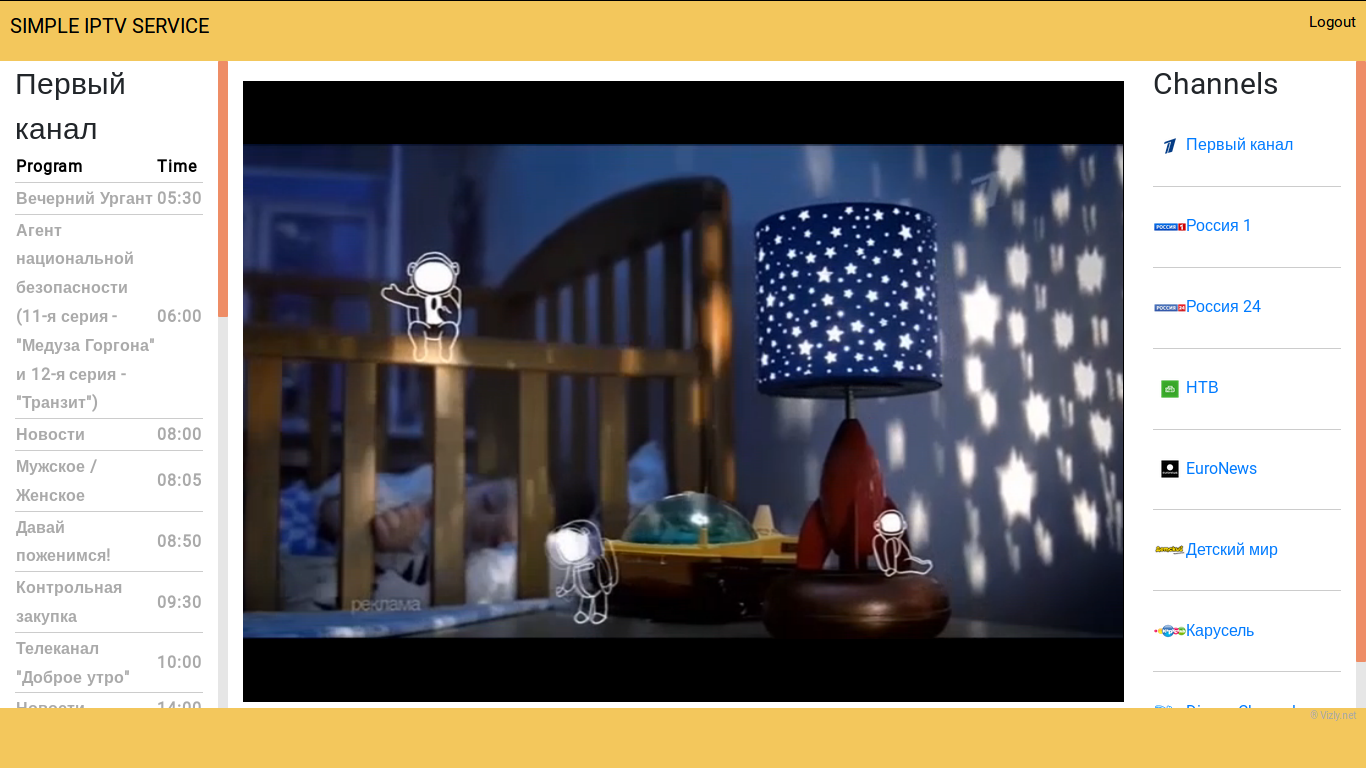
\includegraphics[width=0.45\textwidth]{graphics/web_ui.png}
\caption{Web UI of the prototype}
\label{fig:web_ui}
\end{figure}

